\documentclass[a4paper]{article}

\usepackage{fullpage}

\usepackage{graphicx}
\usepackage{caption}
\usepackage{subcaption}

\usepackage{amsmath}

% Code for typesttting C code
\usepackage{listings}
\usepackage{color}

\definecolor{mygreen}{rgb}{0,0.6,0}
\definecolor{mygray}{rgb}{0.5,0.5,0.5}
\definecolor{mymauve}{rgb}{0.58,0,0.82}
\definecolor{mybrown}{rgb}{0.5,0,0}

\lstdefinestyle{MyCStyle}{ %
  language=C,                      % the language of the code
  backgroundcolor=\color{white},   % choose the background color; you must add \usepackage{color} or \usepackage{xcolor}
  basicstyle=\ttfamily    ,        % the size of the fonts that are used for the code
  breakatwhitespace=false,         % sets if automatic breaks should only happen at whitespace
  breaklines=true,                 % sets automatic line breaking
  captionpos=b,                    % sets the caption-position to bottom
  commentstyle=\color{mygreen},    % comment style
  deletekeywords={...},            % if you want to delete keywords from the given language
  escapeinside={\%*}{*)},          % if you want to add LaTeX within your code
  extendedchars=true,              % lets you use non-ASCII characters; for 8-bits encodings only, does not work with UTF-8
  frame=single,                    % adds a frame around the code
  keepspaces=true,                 % keeps spaces in text, useful for keeping indentation of code (possibly needs columns=flexible)
  keywordstyle=\color{blue},       % keyword style
  morecomment=[l][\color{mybrown}]\#,  % compiler directive
  morekeywords={*,...},            % if you want to add more keywords to the set
  numbers=left,                    % where to put the line-numbers; possible values are (none, left, right)
  numbersep=5pt,                   % how far the line-numbers are from the code
  numberstyle=\tiny\color{mygray}, % the style that is used for the line-numbers
  rulecolor=\color{black},         % if not set, the frame-color may be changed on line-breaks within not-black text (e.g. comments (green here))
  showspaces=false,                % show spaces everywhere adding particular underscores; it overrides 'showstringspaces'
  showstringspaces=false,          % underline spaces within strings only
  showtabs=false,                  % show tabs within strings adding particular underscores
  stepnumber=1,                    % the step between two line-numbers. If it's 1, each line will be numbered
  stringstyle=\color{mymauve},     % string literal style
  tabsize=2,                       % sets default tabsize to 2 spaces
  title=\lstname                   % show the filename of files included with \lstinputlisting; also try caption instead of title
}

\newlength{\pic}

\begin{document}

\title{EE445M Lab 5 Report}
\author{Yen-Kai Huang \\ Siavash Zanganeh Kamali}
\maketitle

\section{Objective} The goal of this lab is to build a working file system. In this lab we will use
low-level library code to interface a SD card, and write the program that serves as a middle-level interface,
with directory access and interpreter commands for easy use. 

As an application of the file system, we will stream the debugging information of a robot onto the SD card.

\section{Software Design} 

\paragraph{(a)} Here is the picture showing the file system scheme we use. It is a linked-list structure
with 32 blocks dedicated to store the directory information.

\setlength{\pic}{0.5\textwidth}
\begin{figure}[htp]
\center
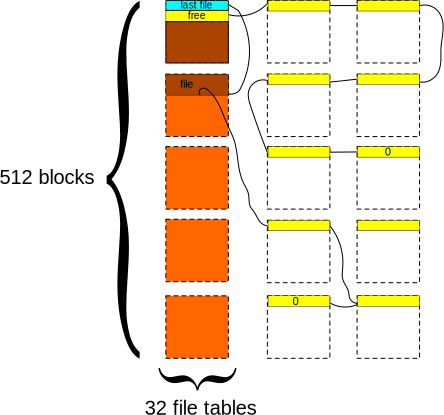
\includegraphics[width=\pic]{drawing}
\end{figure}

The \emph{White} blocks represent file blocks that store actual data. Each of these data blocks has a header
that stores the address of the next blocks in a the same file. If a block is the last in a file this value is \texttt{null}.

The \emph{Orange} and \emph{Brown} parts represent file tables that store the file names, start/end addresses, and size of each file. The first of these file table is special. The first \texttt{short} value is an index of first free spot or the last file among the file tables. The yellow part \emph{free} is a directory object storing the start/end address of the free blocks.

\paragraph{(b) Middle-level File system code}
Below are the file system codes implementing the scheme shown in (a)

\lstset{language=C, style=MyCStyle}
\lstinputlisting{Code/efile.h}

\lstinputlisting{Code/efile.c}

Below is the interpreter commands for easier control of the file system.
\lstinputlisting{Code/interpreter.c}

\section{Measurement}
Below are the data analyzer screen captures.

\setlength{\pic}{8cm}
\begin{figure}[htp]
\center
\begin{subfigure}[H]{\pic}
\includegraphics[width=\pic]{scope/packet}
\end{subfigure}
\\[5pt]
\begin{subfigure}[H]{\pic}
\includegraphics[width=\pic]{scope/packet_zoom}
\end{subfigure}
\caption{Data Analyzer showing packets}
\end{figure}

\paragraph{(1) SD card read bandwidth and write bandwidth by average 10000 blocks\\ }
Writing time = 3153 us/block\\
Reading time = 3169 us/block

\paragraph{(2) SPI clock rate}
The measured SPI clock rate is $100\,ns$\\
The maximum baud rate of SD card is $10\,Mbit$\\

The first picture shows the SPI transmission for the whole communication done for a block write to the SD  Card. The second picture is a zoomed in version of showing the first command sent to write. The microcontroller kept sending empty packets after write, until it received an acknowledge from SD Card that write was done.

\section{Analysis}
\paragraph{1) Does your implementation have external fragmentation? Explain with a one sentence answer.\\}

No, our system uses a linked-list scheme. Therefore it can use all of the data block available and will not have external fragmentation.

\paragraph{2) your disk has ten files, and the number of bytes in each file is a random number, what is the expected 
amount of wasted storage due to internal fragmentation? Explain with a one sentence answer. \\}

In our file system, every data block has the first \texttt{short} used to store the address of the next block.

If the average number of bytes in the files are represented as a random variable $N$,
the block it uses is $B = \lceil \frac{N}{512} \rceil$, and the internal fragmentation is
\begin{equation*}
	2 \times B \times 10 \text{ bytes}
\end{equation*} 

\paragraph{3) Assume you replaced the flash memory in the SD card with a high speed battery-backed RAM and kept all 
other hardware/software the same. What read/write bandwidth could you expect to achieve? Explain with a one 
sentence answer. \\}

The maximum read/write bandwidth would be 100 Mbps. This is the clock frequency of the SPI. Note that we cannot achieve this bandwidth because some bits are used for sending commands and checksums for the SD card.

\paragraph{4) How many files can you store on your disk? Briefly explain how you could increase this number (do not do 
it, just explain how it could have been done). \\}

The maximum number of files is limited by two factors:\\
1- Number of available files in the directory: by $64 \times 31 + 62 = 2046$. \\
2- Number of blocks formatted other than directory = $2^11 - 32= 2016$ \\
\\
In our case, since the number of files is limited by the number of formatted blocks, we can increase the number of files by formatting a larger amount of space in SD card. If the number of available files in the directory is the limiting factor, we should allocate more blocks to the directory.

\paragraph{5) Does your system allow for two threads to simultaneously stream debugging data onto one file? If yes, 
briefly explain how you handled the thread synchronization. If not, explain in detail how it could have been done. 
Do not do it, just give 4 or 5 sentences and some C code explaining how to handle the synchronization. \\}

Our system does not allow multiple threads to stream data into one file. If a thread interrupts the \texttt{eFile\_Write()} function call of another thread there could be errors.

If we wanted to do it, it could be done by adding mutex semaphores into Write function. For an easy solution, we could specify that only one thread should open the file and closes the file. The other thread should wait for the first thread to open the file.

{ \lstset{language=C, frame=none, numbers=none}
\begin{lstlisting}
int eFile_Write (char data) {
	OS_bWait (&Sema4FileWrite);
	
	//The actual code
	
	OS_Signal (&Sema4FileWrite);
}

\end{lstlisting}
}

To safely allow multiple calls to WOpen from each thread, 
{ \lstset{language=C, frame=none, numbers=none}
\begin{lstlisting}
int eFile_WOpen (char data) {
	static char numFileOpen = 0;
	OS_bWait (&Sema4FileWOpen);
	numFileOpen ++;
	if (numFileOpen) {
		//actually open the file
	} 	//Otherwise file is already opened
	
	OS_Signal (&Sema4FileWOpen);
}
int eFile_WClose () {
	static char numFileClose = 0;
	OS_bWait (&Sema4FileWClose);
	numFileOpen --;
	if (numFileOpen == 0) {
		//actually close the file
	} 	//Otherwise some other thread is still writing
	
	OS_Signal (&Sema4FileWClose);
}

\end{lstlisting}
}

% stuff after this point will not show up
\end{document}
